\section{Processamento de Dados}
\subsection{Desigualdade do Processamento de Dados}

\begin{frame}%[allowframebreaks]
  \frametitle{Desigualdade do Processamento de Dados}
  Dada uma fonte de informação, é possível utilizar alguma forma de processamento de dados
  de forma a obter mais informação sobre esta fonte?

  \begin{figure}[h!]
  \centering
  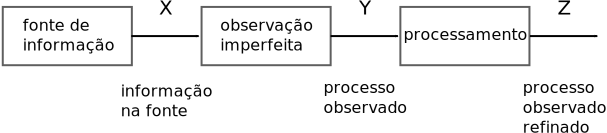
\includegraphics[width=0.8\textwidth]{images/proc-data.pdf}
  %\caption{.}
  \label{fig:proc-data}
  \end{figure} 
\end{frame}

\begin{frame}%[allowframebreaks]
  \frametitle{Desigualdade do Processamento de Dados}
  \begin{itemize}
  \item Imagens com ISO elevado são ruidosas, mas são a única forma de obtermos uma foto
        em baixa luminosidade com pequena abertura (ampla profundidade de campo).
  \item O objetivo da remoção de ruído é recuperar a imagem original.
  \end{itemize}

  \begin{figure}[h!]
  \centering
  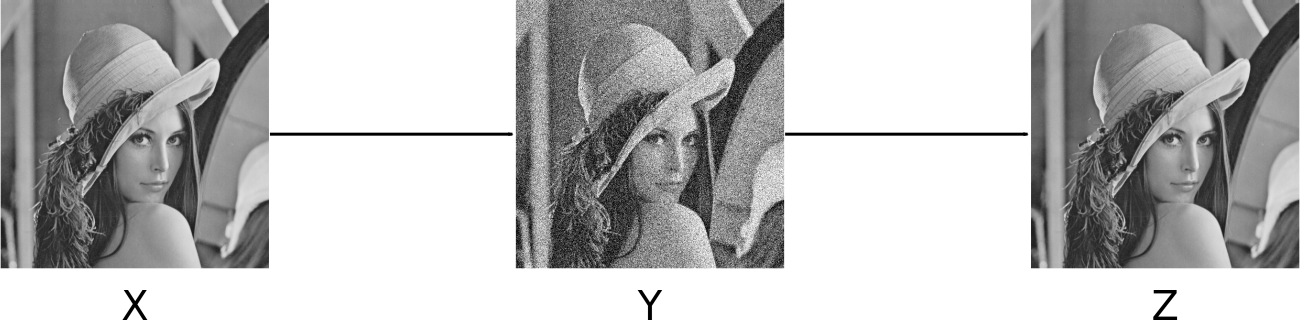
\includegraphics[width=0.8\textwidth]{images/lena-denoising.png}
  %\caption{.}
  \label{fig:lena-denoising}
  \end{figure}

  \begin{itemize}
  \item É possível obter mais informação sobre uma fonte através de processamento adicional?
  \pause
  Infelizmente não.
  \end{itemize}
\end{frame}
\note{
Profundidade de campo descreve até que ponto objetos que estão mais ou menos perto do plano de foco aparentam estar nítidos. 

Regra geral, quanto menor for a abertura do diafragma/íris (maior o valor f/x), para uma mesma distância do objecto fotografado, maior será a distância do plano de foco a que os objetos podem estar enquanto permanecem nítidos.
}

\subsection{Cadeia de Markov}
\begin{frame}[allowframebreaks]
  \frametitle{Cadeia de Markov}
  \begin{definition}[Cadeia de Markov]
  As variáveis aleatórias $X$, $Y$ e $Z$ formam uma cadeia de Markov nesta ordem
  (denotado $X \rightarrow Y \rightarrow Z$) se a distribuição condicional de $Z$
  depende apenas de $Y$ e é condicionalmente independente de $X$. Especificamente,
  $X$, $Y$ e $Z$ formam uma cadeia de Markov $X \rightarrow Y \rightarrow Z$ se
  a função massa de probabilidade conjunta pode ser escrita como
  \begin{equation}
  p(x,y,z) = p(x) p(y|x) p(z|y)
  \end{equation}
  \end{definition}

  \begin{itemize}
  \item $X \rightarrow Y \rightarrow Z$ sse $X$ e $Z$ são condicionalmente independentes
  dado $Y$ ($X \independent Z | Y$). Isto é,
  \begin{equation}
  p(x,z|y) = \frac{p(x,y,z)}{p(y)} = \frac{p(x)p(y|x)p(z|y)}{p(y)} = p(x|y) p(z|y) \ \ \forall x,y,z
  \end{equation}
  \end{itemize}

  \framebreak

  \begin{itemize}
  \item $X \rightarrow Y \rightarrow Z$ implica em $Z \rightarrow Y \rightarrow X$
  \end{itemize}
  \begin{proof}
  \begin{eqnarray}
        p(x,y,z) &=& p(x)p(y|x)p(z|y) = p(x,y)p(z|y) \nonumber \\
                &=& \frac{p(x,y)p(z|y)p(y)}{p(y)} = p(x|y) p(y,z) \nonumber \\
                &=& p(x|y) p(y|z) p(z)
  \end{eqnarray}
  \end{proof}

  \begin{figure}[h!]
  \centering
  
\includegraphics[width=0.8\textwidth]{images/chainxyz.pdf}
  %\caption{.}
  \label{fig:chain}
  \end{figure}

  \begin{itemize}
  \item Se $Z=f(Y)$, então $X \rightarrow Y \rightarrow Z$ (i.e., $X$, $Y$ e $Z$ formam
        uma cadeia de Markov). $f(\cdot)$ pode ser aleatória ou determinística. 
        $X$ é irrelevante para determinar $Z$ quando $Y$ é dado.
  \end{itemize}
\end{frame}

\begin{frame}[allowframebreaks]
  \frametitle{Desigualdade do Processamento de Dados}
  \begin{theorem}[Desigualdade do Processamento de Dados]
   Se $X \rightarrow Y \rightarrow Z$ então
  \begin{equation}
        I(X;Y) \geq I(X;Z)
  \end{equation}
  \end{theorem}
  \begin{itemize}
  \item Na cadeia de Markov, as setas correspondem ao processamento e as variáveis aleatórias 
        correspondem aos dados.
  \item O processamento pode ser aleatório ou determinístico.
  \item A desigualdade de processamento de dados diz que ao efetuar mais processamento dos dados,
        só é possível perder informação sobre a fonte original, quando medida pela informação mútua.
  \end{itemize}

  \framebreak

  \begin{proof}
  Utilizando a regra da cadeia da informação mútua, teremos
  \begin{eqnarray}
  I(X;Y,Z) &=& I(X;Z) + I(X;Y|Z) \nonumber \\
        &=& I(X;Y) + I(X;Z|Y)
  \end{eqnarray}
  Como $X \independent Z |Y$ ($X$ e $Z$ são condicionalmente independentes, dado $Y$), temos
  que $I(X;Z|Y)=0$. Como $I(X;Y|Z) \geq 0$, teremos
  \begin{equation}
  I(X;Z) + \underbrace{I(X; Y|Z)}_{\geq 0} = I(X;Y) + \bcancelto{0}{I(X;Z|Y)}
  \end{equation}
  Então
  \begin{equation}
  I(X;Z) \leq I(X;Y)
  \end{equation}
  \end{proof}

  \begin{itemize}
  \item Teremos igualdade sse $I(X;Y|Z)=0$ (i.e. $X \rightarrow Z \rightarrow Y$).
  \item De forma similar, podemos mostrar que $I(Y;Z) \geq I(X;Z)$.
  \end{itemize}

  \begin{corollary}
   Se $Z=g(Y)$, então $I(X;Y) \geq I(X;g(Y))$.

  Demonstração: $X \rightarrow Y \rightarrow g(Y)$ forma uma cadeia de Markov.
  \end{corollary}

  \begin{corollary}
  Se $X \rightarrow Y \rightarrow Z$ então $I(X;Y|Z) \leq I(X;Y)$.

  \begin{equation}
  \underbrace{I(X;Z)}_{\geq 0} + I(X; Y|Z) = I(X;Y) + \bcancelto{0}{I(X;Z|Y)}
  \end{equation}
  então
  \begin{equation}
  I(X; Y|Z) \leq I(X;Y)
  \end{equation}
  \end{corollary}

  \begin{itemize}
  \item Processamento pode apenas perder informação sobre $X$.
        Quando $X$ é a fonte e $Y$ o receptor, nenhum processamento irá aumentar a informação sobre $X$.
  \item Considere o reconhecimento de padrões: $X$ é um objeto, $Y$ é uma lista de características
        e $f(Y)$ é processamento subsequente. Então, qualquer processamento subsequente poderá apenas
        reduzir a informação sobre o objeto.
  \item Como funciona então as técnicas de remoção de ruído em imagens ou áudio?
        \begin{itemize}
        \item  As técnicas supõem o conhecimento de algumas informações sobre a imagem original, ou seja,
          utilizam conhecimento \textit{a priori} para processar a imagem. 
        \end{itemize}
  \end{itemize}
  
  \begin{corollary}
  Se $X \rightarrow Y \rightarrow Z$, então $I(X; Y|Z) \leq I(X;Y)$. I.e.,
  $I(X; Y|Z) = H(X|Z) - H(X|Y,Z) \leq H(X) - H(X|Y)$.
  \end{corollary}
  
\end{frame}



